\chapter{Технологический раздел}

\section{Язык программирования}
В качестве языка программирований выбран язык высокого уровня JavaScript.

\section{Примеры кода}

\begin{lstlisting}[caption={Частотный побитовый тест}]
function frequencyBitwiseTest(str) {

    let s = 0;
    let n = str.length;

    for (let i = 0; i < n; ++i) {
        if (str[i] == "1")
            ++s;
        else
            --s;
    }

    let sobs = Math.abs(s) / Math.sqrt(n);

    let p = erfc(sobs / Math.sqrt(2));

    return p > 0.01;
}
\end{lstlisting}

\begin{lstlisting}[caption={Тест на одинаковые идущие подряд биты}]
function identicalConsecutiveBitstest(str) {
    let s = 0;
    let n = str.length;

    for (let i = 0; i < n; ++i)
        if (str[i] == "1")  
            ++s;

    let pi = s / n;

    if (Math.abs(pi - 1/2) >= 2 / Math.sqrt(n)) return false;

    let v = 1;

    for (let i = 1; i < n; ++i)
        if (str[i] != str[i - 1])   
            ++v;

    let p = erfc(Math.abs(v - 2 * n * pi * (1 - pi)) / (2 * pi * (1 - pi) * Math.sqrt(2 * n)));

    return p > 0.01;
}
\end{lstlisting}

\section{Взаимодейсвтие с пользователем}

Взаимодейсвтие с пользователем осуществляется через html страницы, открытые в браузере. В пользовательском интерфесе используются динамические таблицы. 

\begin{figure}
  \centering
  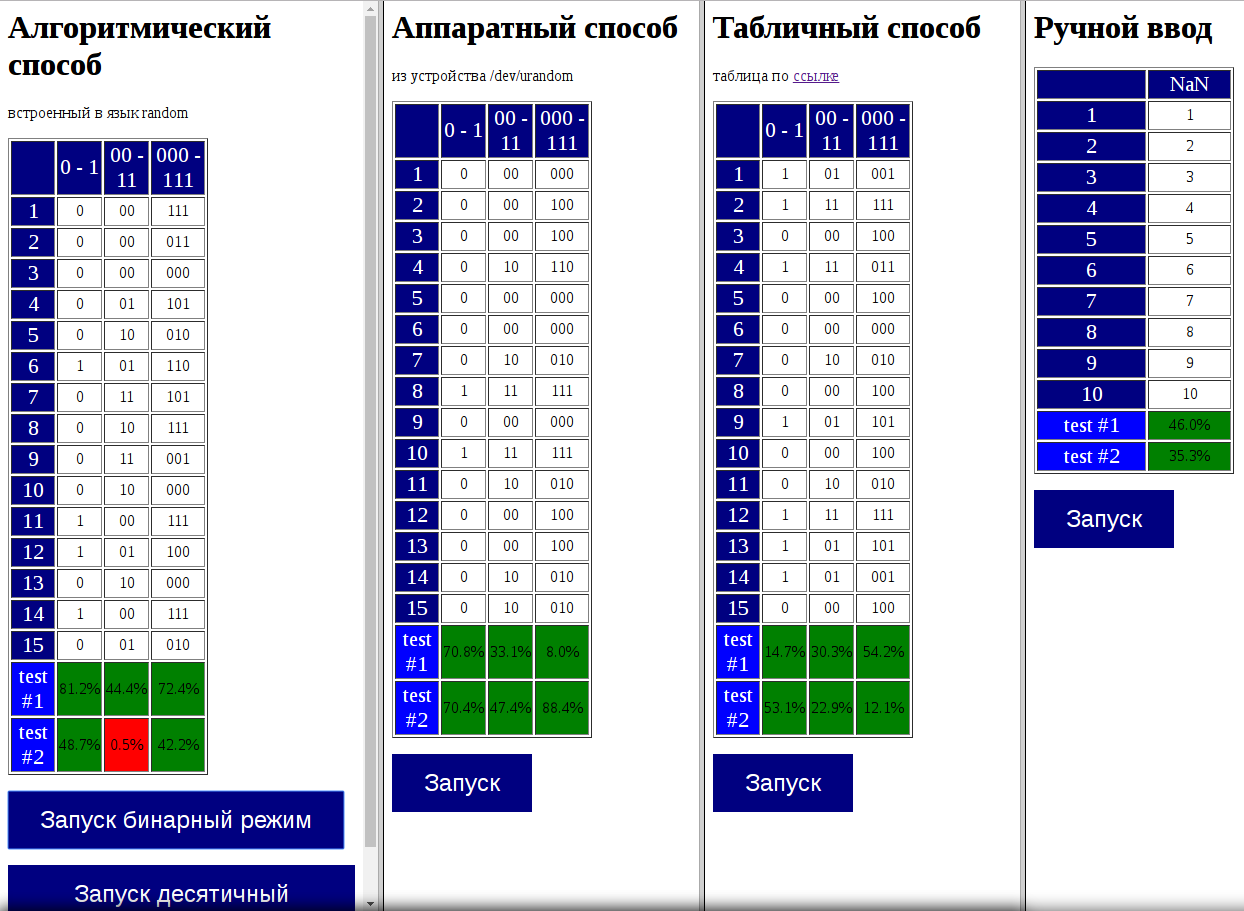
\includegraphics[scale=0.5]{screen1.png}
  \caption{Пример работы программы}
\end{figure}
